\documentclass[english,color,smalltitle]{manchesterposter}
\usepackage{geometry}
\geometry{verbose,landscape,paperwidth=594mm,paperheight=841mm,bmargin=1cm,lmargin=5.5cm,rmargin=1cm,headheight=0cm,headsep=0cm,footskip=0cm}
\setcounter{secnumdepth}{3}
\setcounter{tocdepth}{3}
\usepackage{url}
\usepackage{amsmath}
\usepackage{graphicx}
\usepackage{amssymb}
\usepackage[numbers]{natbib}

\makeatletter

% Use pdflatex to create this poster.


% Sets up colors of bullets.
\AtBeginDocument{
  \def\labelitemi{\color{gold}\ding{122}\color{foreground}}
  \def\labelitemii{\color{gold}\ding{229}\color{foreground}}
}

\makeatother


\begin{document}


\title{Hierarchical Gaussian Process Latent Variable Models}


\author{Neil D. Lawrence \url{neill@cs.man.ac.uk} and Andrew J. Moore \url{A.Moore@dcs.shef.ac.uk}}

\maketitle
\begin{multicols}{5}{\LARGE \par}

\begin{columnbox}
\-

\mysection{Overview}

\medskip{}
The Gaussian process latent variable model (GP-LVM) is a powerful
approach for probabilistic modelling of high dimensional data through
dimensional reduction. In this paper we extend the GP-LVM through
hierarchies. A hierarchical model (such as a tree) allows us to express
conditional independencies in the data as well as the manifold structure.
We first introduce Gaussian process hierarchies through a simple dynamical
model, we then extend the approach to a more complex hierarchy which
is applied to the visualisation of human motion data sets.{\large \par}

\end{columnbox}


\begin{columnbox}
\-

\mysection{Introduction}

\begin{itemize}
\item GP-LVM: an effective to probabilistic modelling of high dimensional
data, assumes it lies on a manifold.{\large \par}
\item An alternative to manifold representations: develop a latent variable
model with sparse connectivity.{\large \par}
\item Example: tree structured models for images \citep{Williams:tree98,Feng:combining02,Awasthi:image07},
object recognition \citep{Felzenszwalb:efficient00,Ioffe:mixtures01}
and human pose estimation \citep{Ramanan:finding03,Sigal:loose04,Lan:beyond05}.{\large \par}
\item Tree structures  offer a convenient way to specify conditional independencies
in the model. {\large \par}
\item We will show how we can construct our dimensionality reduction in
a hierarchical way, exploiting the advantages of expressing conditional
independencies and low dimensional non-linear manifolds.{\large \par}
\end{itemize}
\end{columnbox}


\begin{columnbox}
\-

\mysection{Probabilistic Dimensional Reduction}

\begin{itemize}
\item Formulate a latent variable model, with lower latent than data dimension,
$q<d$. {\large \par}

\begin{itemize}
\item Latent space prior distribution $p\left(\mathbf{X}\right)$. {\large \par}
\item Mapping from latent ($\mathbf{x}_{n}$) to data space ($\mathbf{y}_{n}$)\[
y_{ni}=f_{i}\left(\mathbf{x}_{n};\mathbf{W}\right)+\epsilon_{n},\]
$\mathbf{W}$ is a matrix of mapping parameters. {\large \par}
\end{itemize}
\item For linear mappings and Gaussian priors: recover probabilistic PCA
\citep{Tipping:probpca99}.{\large \par}
\item For non-linear mapping: unclear how to propagate prior distribution
to data space.{\large \par}
\end{itemize}
\end{columnbox}


\begin{columnbox}
\-

\mysection{Dual Approach}

\begin{itemize}
\item Place Gaussian Process prior over the mappings.{\large \par}
\item Marginalise mappings: {\large \par}

\begin{itemize}
\item for linear kernel a dual probabilistic PCA is recovered.{\large \par}
\item for non-linear kernel --- a non linear probabilistic PCA.{\large \par}
\end{itemize}
\end{itemize}
\end{columnbox}


\begin{columnbox}
\-

\mysection{GP-LVM}

\begin{itemize}
\item Several advantages to marginalising the mapping:{\large \par}

\begin{itemize}
\item \emph{e.g.} adding dynamical priors in the latent space \citep{Wang:gpdm05,Urtasun:3dpeople06} {\large \par}
\item constraining points in the latent space \citep{Lawrence:backconstraints06}. {\large \par}
\end{itemize}
\item Here we further exploit this characteristic, proposing the hierarchical
Gaussian process latent variable model{\large \par}
\item Introduce it by simple (one layered) hierarchical model for \emph{dynamics.} {\large \par}
\end{itemize}
\end{columnbox}


\begin{columnbox}
\-

\mysection{Dynamics via a Simple Hierarchy}

\begin{itemize}
\item Standard latent space dynamical prior: $p\left(\mathbf{X}\right)=p\left(\mathbf{x}_{1}\right)\prod_{t=2}^{T}p\left(\mathbf{x}_{t}|\mathbf{x}_{t-1}\right)$. {\large \par}
\item Combine a with the GP-LVM likelihood and seek a \emph{maximum a posteriori}
(MAP) solution.{\large \par}
\item \citet{Wang:gpdm05} \emph{autoregressive} Gaussian process prior
to augment the GP-LVM with dynamics. {\large \par}
\item Consider an \emph{regressive} Gaussian process implementation of dynamics.{\large \par}

\begin{itemize}
\item We place a Gaussian process prior over the latent space, the inputs
are given by the time frame, $\mathbf{t}$. {\large \par}
\item Removes requirement for uniform sampling.{\large \par}
\item Allows the path in latent space to bifurcate.{\large \par}
\end{itemize}
\end{itemize}
\end{columnbox}


\begin{columnbox}
\-

\mysection{Notation}

\begin{itemize}
\item Motion capture sequence, $\mathbf{Y}=\left[\mathbf{y}_{1,:},\dots,\,\mathbf{y}_{T,:}\right]^{\mbox{T}}\in\Re^{T\times d}$ {\large \par}
\item GP-LVM Likelihood\begin{equation}
p\left(\mathbf{Y}|\mathbf{X}\right)=\prod_{j=1}^{d}N\left(\mathbf{y}_{:,j}|\mathbf{0},\mathbf{K}_{x}\right),\label{eq:gplvmLikelihood}\end{equation}
{\large \par}
\item Latent variables, $\mathbf{X}=\left[\mathbf{x}_{1},\dots,\,\mathbf{x}_{T}\right]^{\mbox{T}}\in\Re^{T\times q}$, {\large \par}
\item Kernel Matrix\[
k_{x}\left(\mathbf{x}_{i},\mathbf{x}_{j}\right)=\sigma_{\mbox{rbf}}^{2}\exp\left(-\frac{\left\Vert \mathbf{x}_{i}-\mathbf{x}_{j}\right\Vert ^{2}}{2l_{x}^{2}}\right)+\sigma_{\mbox{white}}^{2}\delta_{ij},\]
{\large \par}
\item Place a prior over the elements of $\mathbf{X}$. \begin{equation}
p\left(\mathbf{X}|\mathbf{t}\right)=\prod_{i=1}^{q}N\left(\mathbf{x}_{:,i}|\mathbf{0},\mathbf{K}_{t}\right),\label{eq:gpTemporalPrior}\end{equation}
 $\mathbf{t}\in\Re^{T\times1}$ is vector of sample times.{\large \par}
\item Kernel Matrix\[
k_{t}\left(t_{i},t_{j}\right)=\varsigma_{\mbox{rbf}}^{2}\exp\left(-\frac{\left(t_{i}-t_{j}\right)^{2}}{2l_{t}^{2}}\right)+\varsigma_{\mbox{white}}^{\mbox{2}}.\]
Samples shown below.{\large \par}
\end{itemize}
\end{columnbox}


\begin{columnbox}
\-

\mysection{Regressive Dynamics}

%
\begin{minipage}[c][1\totalheight]{1\columnwidth}%
\begin{center}
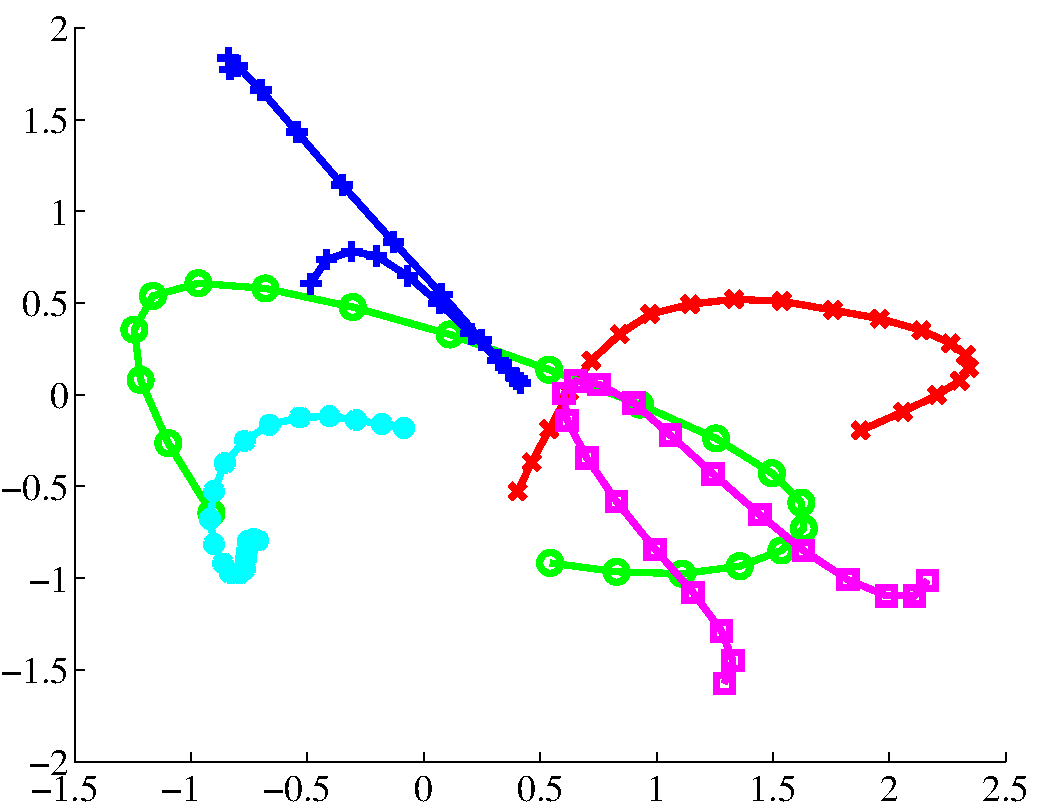
\includegraphics[width=0.8\columnwidth]{./diagrams/demTemporalSamplePaths}
\par\end{center}{\LARGE \par}

\begin{center}
\small Typical sample paths for the RBF covariance function as temporal
prior over the latent space.\label{fig:Typical-sample-paths}
\par\end{center}%
\end{minipage}{\large \par}

\end{columnbox}


\begin{columnbox}
\-

\mysection{More Complex Hierarchies\label{sec:complexHierarchies}}

\begin{itemize}
\item This is a simple hierarchy. A Gaussian process prior on the latent
space of a Gaussian process.{\large \par}
\item Can we create more complex hierarchies and still find MAP solutions?{\large \par}
\item We consider a motion capture example with multiple subjects interacting. {\large \par}
\item Use a simple tree structure to model the subjects.{\large \par}
\end{itemize}
\end{columnbox}


\begin{columnbox}
\-

\mysection{Subject Interaction}

%
\begin{minipage}[c][1\totalheight]{1\columnwidth}%
\begin{center}
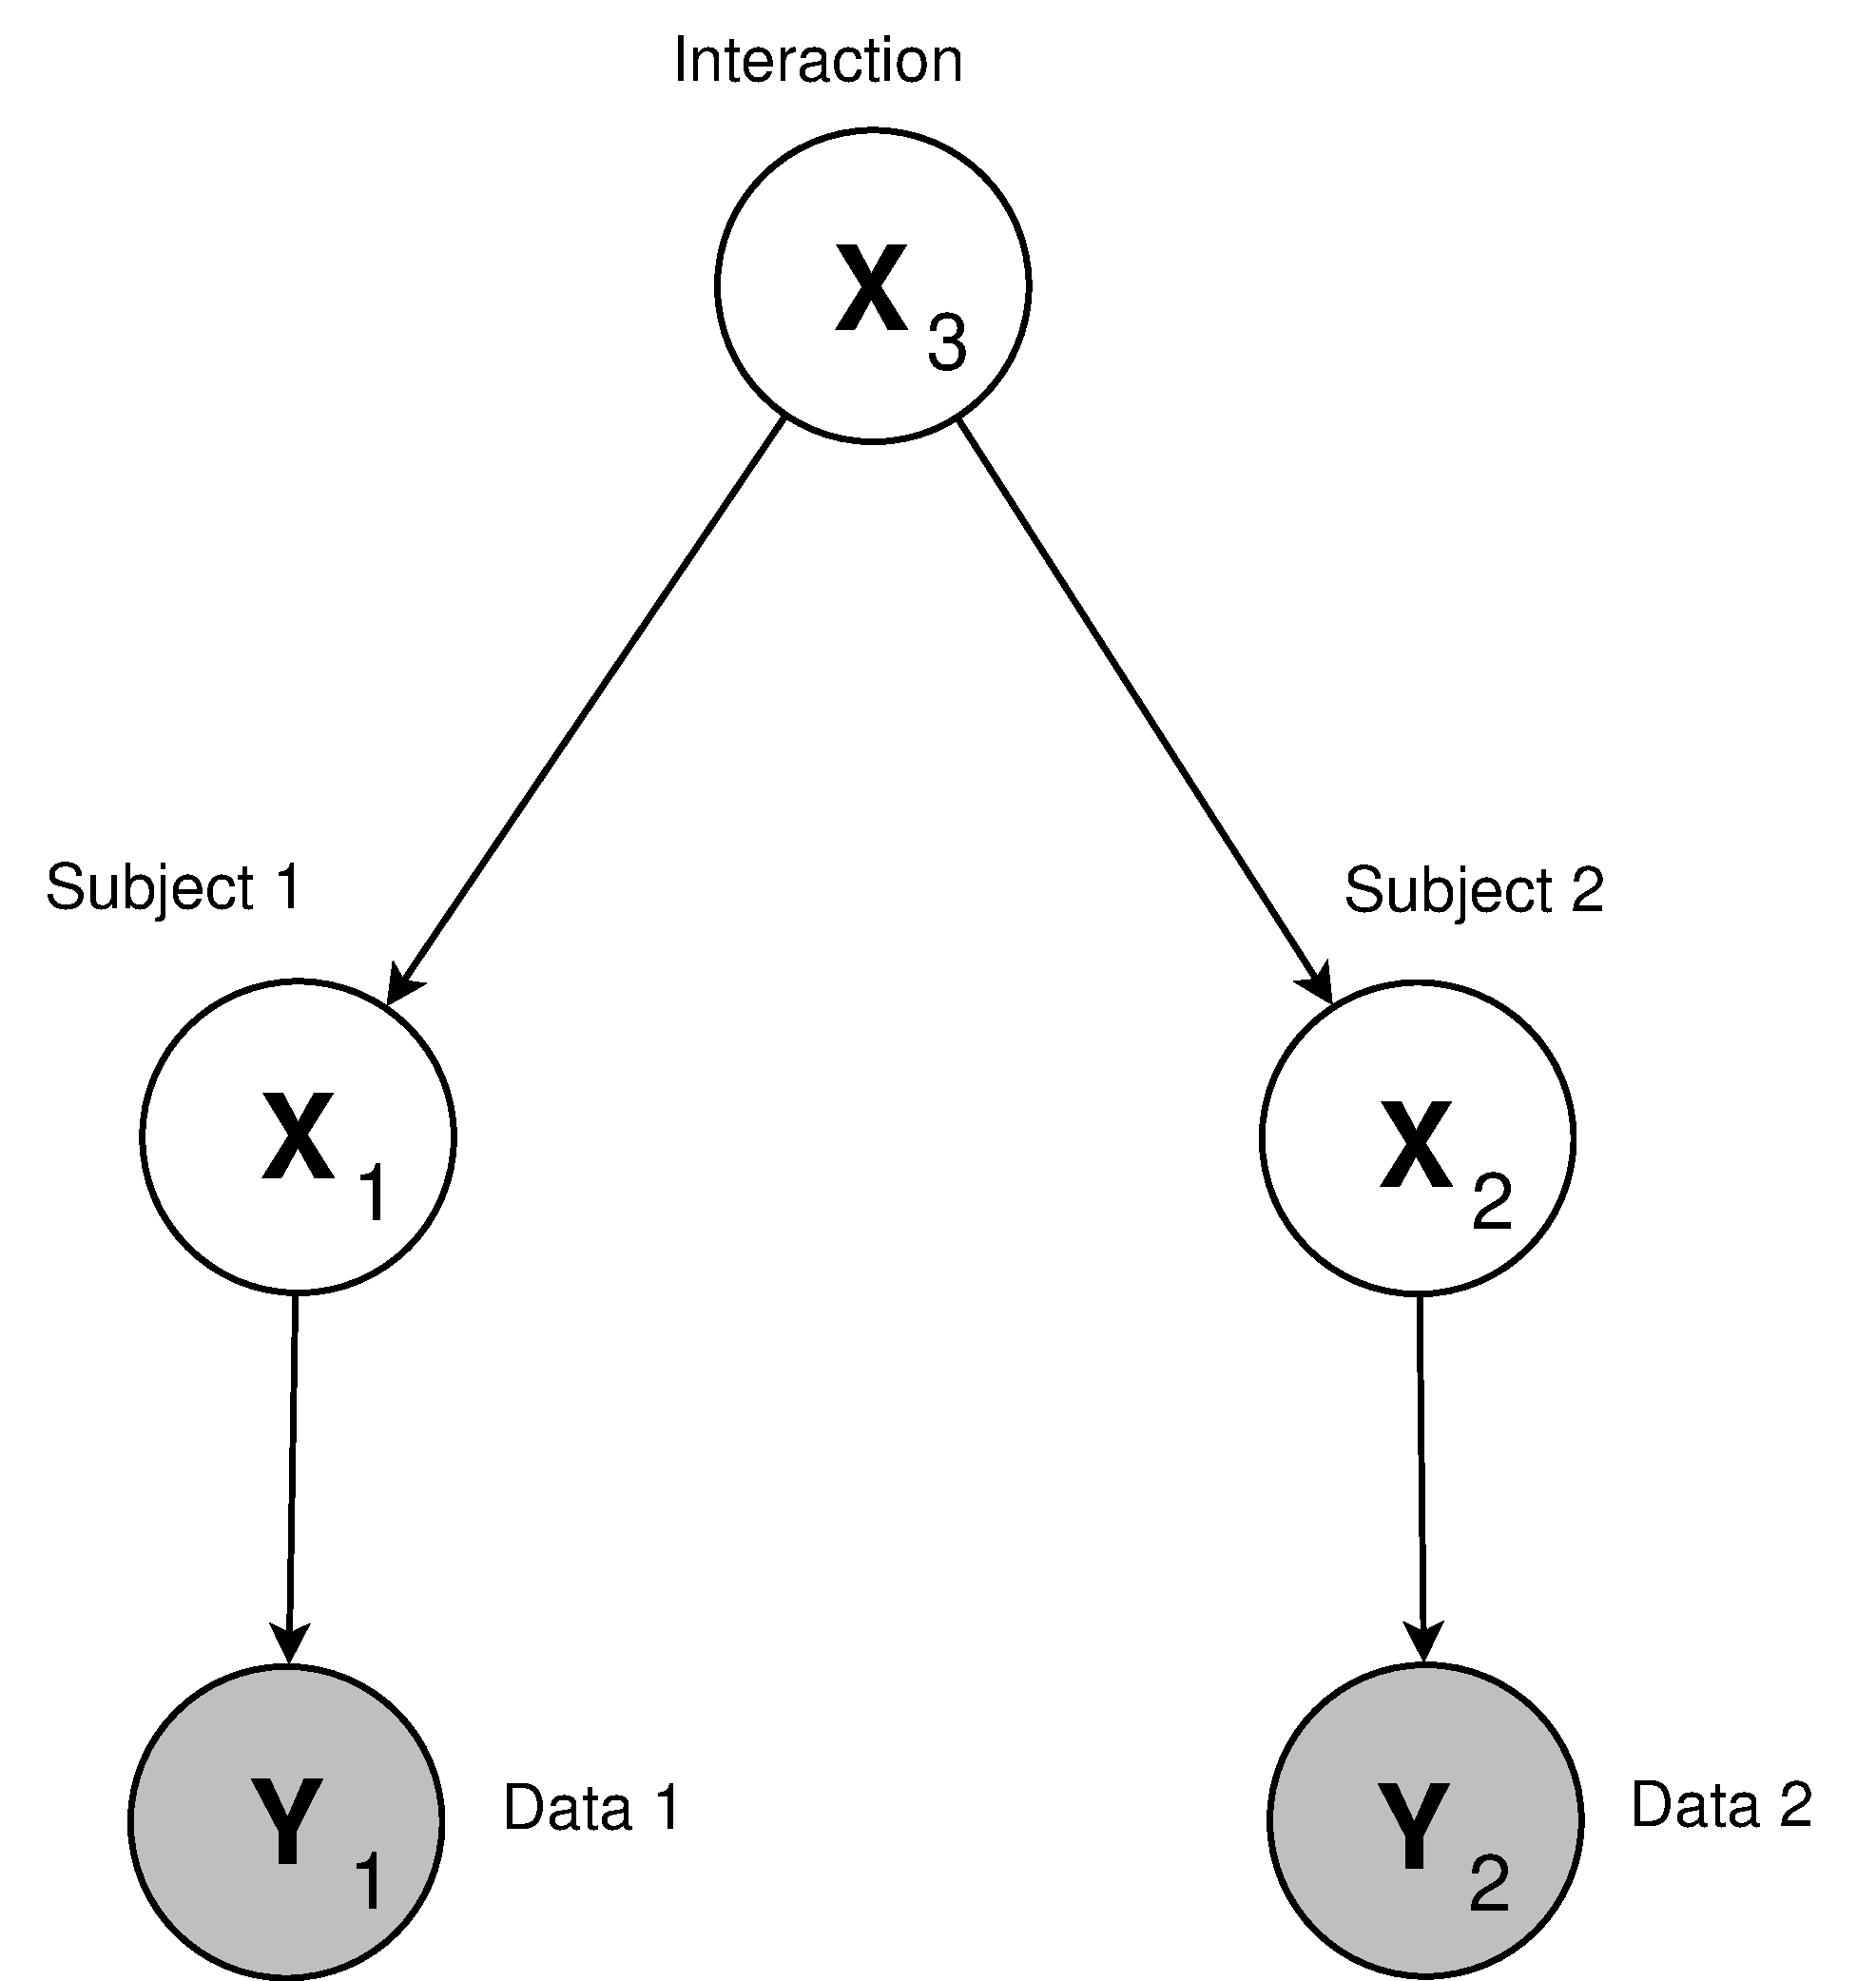
\includegraphics[width=0.7\columnwidth]{./diagrams/twoSubjects}
\par\end{center}{\LARGE \par}

\begin{center}
\small A simple hierarchy for capturing interaction between two subjects
where $\mathbf{Y}_{1}$ is the data associated with subject 1, $\mathbf{Y}_{2}$
is that of subject 2. Each of these variable sets is then controlled
by latent variables, $\mathbf{X}_{1}$ and $\mathbf{X}_{2}$. These
latent variables are in turn controlled by $\mathbf{X}_{3}$. \label{fig:twoSubjects}
\par\end{center}%
\end{minipage}{\large \par}

\end{columnbox}


\begin{columnbox}
\-

\mysection{Joint Probability}

\begin{itemize}
\item The joint probability: \[
p\left(\mathbf{Y}_{1},\mathbf{Y}_{2}\right)=\int p\left(\mathbf{Y}_{1}|\mathbf{X}_{1}\right)\int p\left(\mathbf{Y}_{2}|\mathbf{X}_{2}\right)\int p\left(\mathbf{X}_{1},\mathbf{X}_{2}|\mathbf{X}_{3}\right)\mbox{d}\mathbf{X}_{3}\mbox{d}\mathbf{X}_{2}\mbox{d}\mathbf{X}_{1}\]
{\large \par}
\item Has an intractable integral. {\large \par}
\item We therefore turn to MAP solutions for finding the values of the latent
variables. {\large \par}
\item Maximise\begin{eqnarray*}
\log p\left(\mathbf{X}_{1},\mathbf{X}_{2}\mathbf{X}_{3}|\mathbf{Y}_{1},\mathbf{Y}_{2}\right) & = & \log p\left(\mathbf{Y}_{1}|\mathbf{X}_{1}\right)+\log p\left(\mathbf{Y}_{2}|\mathbf{X}_{2}\right)+\log p\left(\mathbf{X}_{1},\mathbf{X}_{2}|\mathbf{X}_{3}\right)\end{eqnarray*}
first two terms for the subjects, third term provides coordination.{\large \par}
\end{itemize}
\end{columnbox}


\begin{columnbox}


\mysection{Two Interacting Subjects}

\begin{itemize}
\item MOCAP data%
\footnote{\url{http://mocap.cs.cmu.edu}.%
} consists of two subjects that `high five'. {\large \par}
\item The algorithm for optimisation of the latent variables proceeded as
follows:{\large \par}

\begin{enumerate}
\item Initialise each leaf node's latent variable set ($\mathbf{X}_{1},\mathbf{X}_{2}$)
through PCA of corresponding data set ($\mathbf{Y}_{1}$,$\mathbf{Y}_{2}$).{\large \par}
\item Initialise the root node's latent variable set ($\mathbf{X}_{3}$)
through PCA of concatenated latent variables of dependents $\left[\mathbf{X}_{1}\,\,\mathbf{X}_{2}\right]$.{\large \par}
\item Optimise jointly the kernel parameters and latent positions $\left(\mathbf{X}_{1},\mathbf{X}_{2},\mathbf{X}_{3}\right)$. {\large \par}
\end{enumerate}
\item Used a variable sample rate to capture fast hand movements.{\large \par}
\item The variable sample rate presents no problems for our regressive dynamics.{\large \par}
\end{itemize}
\end{columnbox}


\begin{columnbox}
\-

\mysection{Interacting Subjects}

%
\begin{minipage}[c][1\totalheight][t]{1\columnwidth}%
\begin{center}
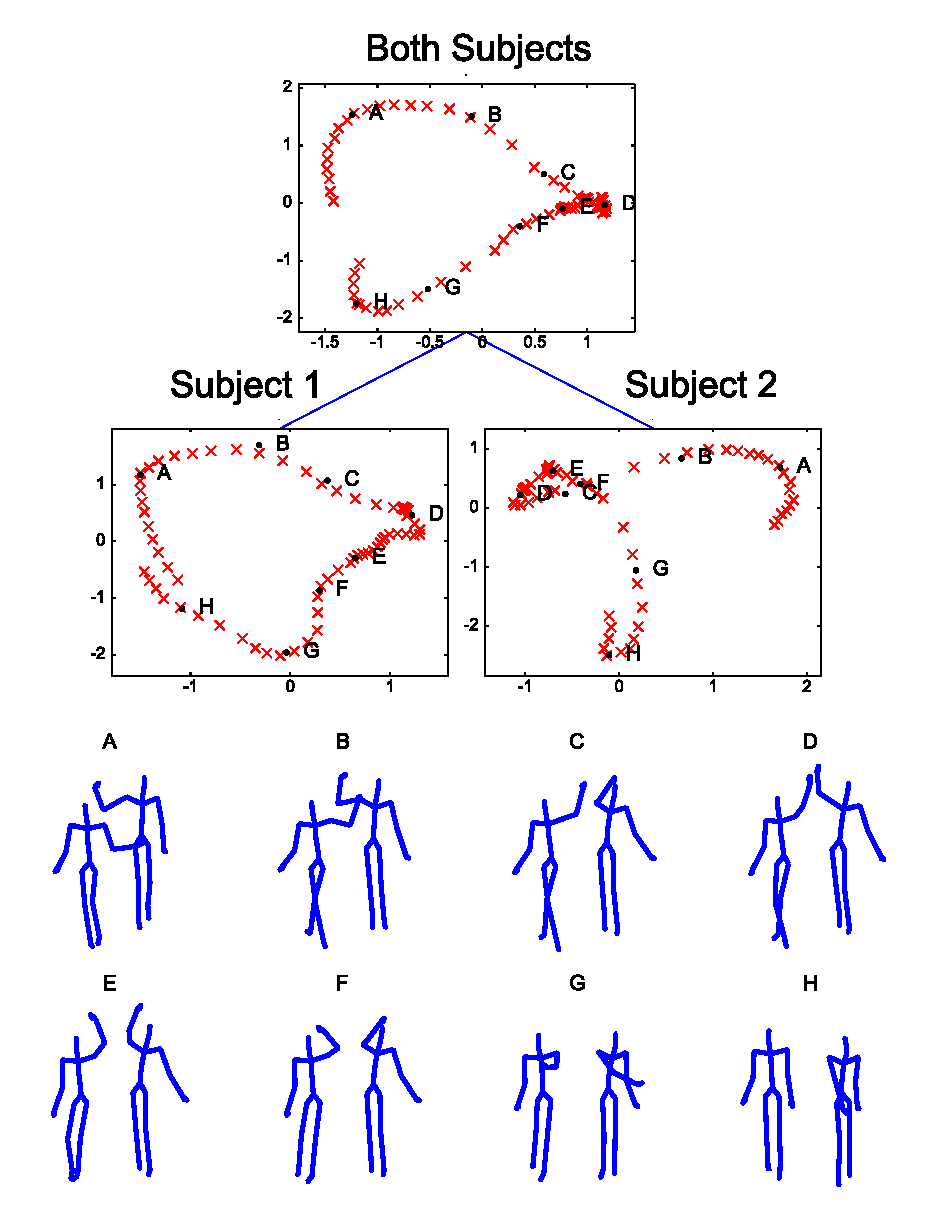
\includegraphics[width=1\columnwidth]{./diagrams/demHighFive_icml}
\par\end{center}{\LARGE \par}

\small High Five example. Two subjects are modelled as they walk
towards each other and `high five'. Plot shows the simple hierarchy
used to model the data. There is a regressive dynamical prior placed
over the latent space of the root node. The root node then controls
the two individual subjects. To illustrate the model we have taken
points at time (i.e we input these values of $t$ into the dynamical
model) frames A: 85, B: 114, C:127, D: 141, E: 155, F: 170, G: 190
and H: 215. These points mapped down through the hierarchy and into
the data space. In each of the plots of the two subjects, Subject
1 is on the right and Subject 2 is on the left. \label{fig:highFive}%
\end{minipage}{\large \par}

\end{columnbox}


\begin{columnbox}
\-

\mysection{Subject Decomposition}

\begin{itemize}
\item We can also consider decomposition of a single subject into parts. {\large \par}
\item Most tree based approaches to mocap modelling assume the nodes are
observed and the tree reflects skeletal structure.{\large \par}
\item Our hierarchical model is more similar to \citep{Williams:tree98}
where the tree structure is a \emph{hierarchy of latent variables}. {\large \par}
\end{itemize}
\end{columnbox}


\begin{columnbox}
\-

\mysection{Skeleton Decomposition}

%
\begin{minipage}[t][1\totalheight]{1\columnwidth}%
\begin{center}
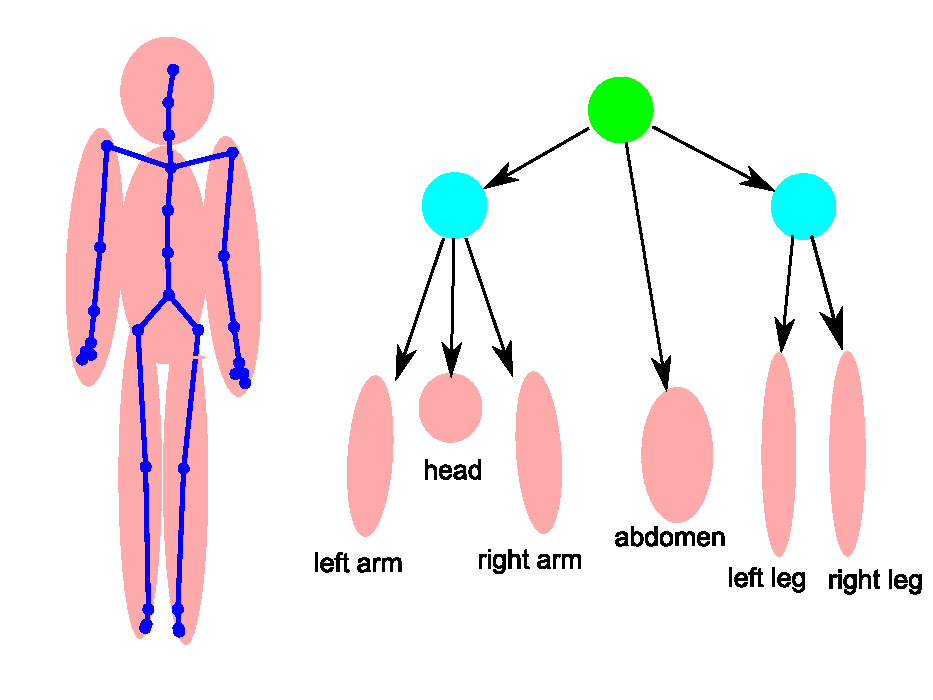
\includegraphics[width=0.9\columnwidth]{./diagrams/stickHierarchy}
\par\end{center}{\LARGE \par}

\small Decomposition of skeleton for hierarchical modelling. By separating
the component parts of the skeleton in this manner we can model the
space of natural motions for each component part and express them
independently or jointly.\label{fig:skeletonDecomposition}%
\end{minipage}{\large \par}

\end{columnbox}


\begin{columnbox}
\-

\mysection{Decomposition in a Walk and Run}

\begin{itemize}
\item Data set composed of a walking motion and a running motion.{\large \par}
\item Data sub-sampled to 30 frames per second and one cycle of each motion
was used. {\large \par}
\item We modelled the subject using the decomposition shown in above.{\large \par}
\item To reflect the fact that two different motions were present in the
data we constructed a hierarchy with \emph{two roots}. One for the
run and one for the walk.{\large \par}
\item This construction enables us to express the two motion sequences separately
while sharing information lower in the hierarchy.{\large \par}
\item We used a periodic kernel for the regressive dynamics. {\large \par}
\end{itemize}
\end{columnbox}


\begin{columnbox}
\-

\mysection{Decomposition Result}

%
\begin{minipage}[t][1\totalheight]{1\columnwidth}%
\begin{center}
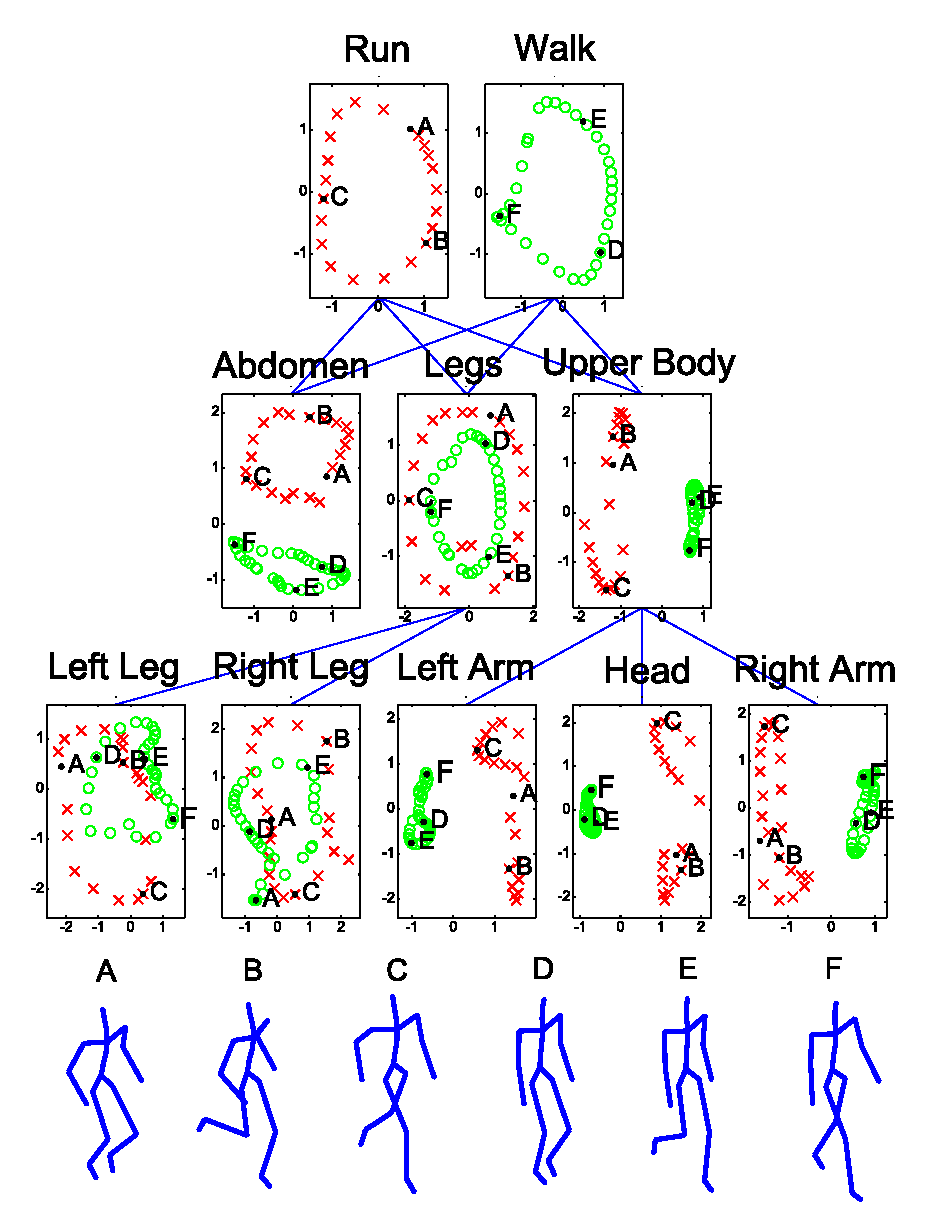
\includegraphics[width=1\textwidth]{./diagrams/demWalkRun_icml}
\par\end{center}{\LARGE \par}

\small Combined model of a run and a walk. The skeleton is decomposed
as shown in Figure~\ref{fig:skeletonDecomposition}. In the plots,
crosses are latent positions associated with the run and circles are
associated with the walk. We have mapped three points from each motion
through the hierarchy. Periodic dynamics was used in the latent spaces.\label{fig:demRunWalk1}%
\end{minipage}{\large \par}

\end{columnbox}


\begin{columnbox}
\-

\mysection{Summary}

\begin{itemize}
\item Introduced a a hierarchical version of the GP-LVM{\large \par}
\item We use MAP approximations to fit latent variables in all different
levels of the hierarchy.{\large \par}
\end{itemize}
\end{columnbox}


\begin{columnbox}
\-

\mysection{Overfitting}

\begin{itemize}
\item GP-LVM uses a large number of `parameters' in the form of latent points.
Why doesn't it overfit?{\large \par}
\item Standard GP-LVM: parameters increase linearly $\frac{q}{d}\times N$.
If $q<d$ overfitting not a problem.{\large \par}
\item HGP-LVM: we are adding more latent variables, will we overfit? {\large \par}

\begin{itemize}
\item Upper levels of hierarchy only regularise the leaf nodes: if the leaf
nodes don't overfit neither will the model.{\large \par}
\item By modifying the locations of latent variables we are changing the
\emph{regularisation} of the leaf nodes.{\large \par}
\item If unconstrained the model would simply remove the regularisation.{\large \par}
\item We counter this potential problem in two ways. {\large \par}

\begin{enumerate}
\item Provided a fixed dynamical prior at the top level. {\large \par}
\item Constrained the noise variance of each non-leaf Gaussian process to
$1\times10^{-6}$.{\large \par}
\end{enumerate}
\end{itemize}
\end{itemize}
\end{columnbox}


\begin{columnbox}
\-

\mysection{Other Hierarchical Models}

\begin{itemize}
\item The model is not closely related to hierarchical PCA \citep{Bishop:hierarchy98}.{\large \par}
\item Hierarchical PCA the hierarchy is not a hierarchy of latent variables
but a hierarchical decomposition of the component probabilities.{\large \par}
\end{itemize}
\end{columnbox}


\begin{columnbox}
\-

\mysection{Applications}

\begin{itemize}
\item Two application areas of promise are:{\large \par}

\begin{itemize}
\item Tracking: GP-LVM is used as a prior model in tracking, the hierarchy
would allow different components to be swapped in as motion changed
and `back off'. {\large \par}
\item Animation: animator time is expensive. Through combining the hierarchical
model with style based inverse kinematics \citep{Grochow:styleik04}
these costs could be reduced. {\large \par}
\end{itemize}
\end{itemize}
\end{columnbox}


\begin{columnbox}
\-

\mysection{Acknowledgments\medskip{}
}

{\footnotesize This work was funded by the EU FP6 PASCAL Network of
Excellence under a pump priming grant. The motion capture data used
in this project was obtained from }\texttt{\footnotesize mocap.cs.cmu.edu}{\footnotesize .
The database was created with funding from NSF EIA-0196217. We thank
Raquel Urtasun for helpful discussions.}{\footnotesize \par}

\end{columnbox}


\begin{columnbox}
\-

\mysection{Recreating the Experiments}

\medskip{}
{\footnotesize The source code for re-running all the experiments
detailed here is available from \url{http://www.cs.man.ac.uk/~neill/hgplvm/},
release 0.1. }{\footnotesize \par}

\end{columnbox}


\begin{columnbox}
\-

{\footnotesize \bibliographystyle{abbrvnat_notitle}
\bibliography{manchesterPosterExample}
}{\footnotesize \par}

\end{columnbox}


\end{multicols}

\end{document}
